\documentclass{article}
\usepackage{amsmath,amsfonts,amsthm,amssymb,amsopn,bm}
\usepackage[margin=.9in]{geometry}
\usepackage{graphicx}
\usepackage{url}
\usepackage[usenames,dvipsnames]{color}
\usepackage{fancyhdr}
\usepackage{multirow}
\usepackage{listings}
\usepackage{hyperref}

\definecolor{keywords}{RGB}{255,0,90}
\definecolor{comments}{RGB}{0,0,113}
\definecolor{red}{RGB}{160,0,0}
\definecolor{green}{RGB}{0,150,0}
 
\lstset{language=Python, 
        basicstyle=\ttfamily\tiny, 
        keywordstyle=\color{keywords},
        commentstyle=\color{comments},
        stringstyle=\color{red},
        showstringspaces=false}

\newcommand{\argmax}{\arg\!\max}
\newcommand{\argmin}{\arg\!\min}
\newcommand{\field}[1]{\mathbb{#1}}
\newcommand{\1}{\mathbf{1}}
\newcommand{\E}{\mathbb{E}} 
\renewcommand{\P}{\mathbb{P}}
\newcommand{\R}{\field{R}} % real domain
% \newcommand{\C}{\field{C}} % complex domain
\newcommand{\F}{\field{F}} % functional domain
\newcommand{\T}{^{\textrm T}} % transpose
\def\diag{\text{diag}}

%% operator in linear algebra, functional analysis
\newcommand{\inner}[2]{#1\cdot #2}
\newcommand{\norm}[1]{\left\|#1\right\|}
\newcommand{\twonorm}[1]{\|#1\|_2^2}
% operator in functios, maps such as M: domain1 --> domain 2
\newcommand{\Map}[1]{\mathcal{#1}}
\renewcommand{\theenumi}{\alph{enumi}} 


\newcommand{\Perp}{\perp \! \! \! \perp}

\newcommand\independent{\protect\mathpalette{\protect\independenT}{\perp}}
\def\independenT#1#2{\mathrel{\rlap{$#1#2$}\mkern2mu{#1#2}}}
\newcommand{\vct}[1]{\boldsymbol{#1}} % vector
\newcommand{\mat}[1]{\boldsymbol{#1}} % matrix
\newcommand{\cst}[1]{\mathsf{#1}} % constant
\newcommand{\ProbOpr}[1]{\mathbb{#1}}
\newcommand{\points}[1]{\small\textcolor{magenta}{\emph{[#1 points]}} \normalsize}
\date{{}}

\setlength\parindent{0px}

\begin{document}
\title{Homework \#1 B}
\author{\normalsize{Spring 2020, CSE 446/546: Machine Learning}\\
\normalsize{Dino Bektesevic}}
\maketitle

\section*{Ridge regression on MNIST}
B.2 
\begin{enumerate}
    \item \points{10} We just fit a classifier that was linear in the pixel intensities to the MNIST data. For classification of digits the raw pixel values are very, very bad features: it’s pretty hard to separate digits with linear functions in pixel space. The standard solution to this is to come up with some transform $h:\R^d\rightarrow \R^p$ of the original pixel values such that the transformed points are (more easily)linearly separable. In this problem, you’ll use the feature transform:
    
    $$h(x) = \cos(Gx+b)$$
    
    where $G\in R^{p\times d}$, $b\in \R^p$, and the cosine function is applied element wise. We’ll choose $G$ to be a random matrix, with each entry sampled i.i.d. from a Gaussian with mean $\mu = 0$ and variance $\sigma^2=0.1$, and $b$ to be a random vector sampled i.i.d. from the uniform distribution on $[0, 2\pi]$. The big question is: how do we choose $p$? Using cross-validation, of course! Randomly partition your training set into proportions 80/20 to use as a new training set and validation set, respectively. Using the train function you wrote above, train $\widehat W_p$ for different values of $p$ and plot the classification training error and validation error on a single plot with $p$ on the x-axis. Be careful, your computer may run out of memory and slow to a crawl if $p$ is too large ($p\leq 6000$ should fit into 4 GB of memory that is a minimum for most computers, but if you’re having trouble you can set $p$ in the several hundreds). You can use the same value of $\lambda = 1e-4$ as above but feel free to study the effect of using different values of $\lambda$ and $\sigma^2$ for fun.
    
    \begin{center}
        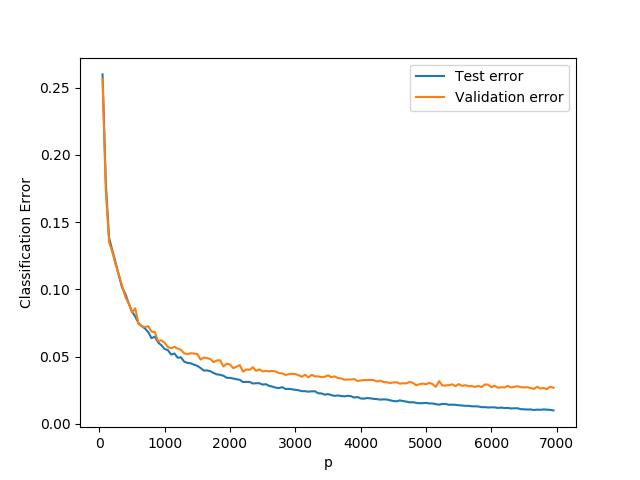
\includegraphics[width=4in]{HW1/HW1_plots/ClassificationError.png}
    \end{center}    
    
\begin{lstlisting}[language=Python]
import numpy as np
from scipy import linalg
import matplotlib . pyplot as plt

from mnist import MNIST


def load_mnist_dataset(path="data/mnist_data/"):
    """Loads MNIST data located at path.

    MNIST data are 28x28 pixel large images of letters.

    Parameters
    ----------
    path : `str`
        path to the data directory

    Returns
    -------
    train : `np.array`
        train data normalized to 1
    trainlabels : `np.array`
        train data labels
    test : `np.array`
        test data normalized to 1
    testLabels : `np.array`
        test data labels
    """
    mndata = MNIST("data/mnist_data/")

    train, trainLabels = map(np.array, mndata.load_training())
    test, testLabels  = map(np.array, mndata.load_testing())

    train = train/255.0
    test = test/255.0

    return train, trainLabels, test, testLabels


def one_hot(length, index):
    """Given an index and length k returns an array where all elements are zero
    except the one at index location, where the value is 1.

    Parameters
    ----------
    length : `int`
        Length of the almost-zero array.
    index : `int`
        Index at which element value is set to 1

    Returns
    -------
    arr : `np.array`
        Array of zeros except for arr[index]=1.
    """
    arr = np.zeros(length)
    arr[index] = 1
    return arr


def train(X, Y, lamb):
    """Given data, labels and regularization constant lambda solves

    $$ W = (X^T X) + \lambda I $$

    to retrieve weights of our model.

    Parameters
    ----------
    X : `np.array`
        Data to fit to
    Y : `np.array`
        Data labes, a length 10 array where index of element with value 1 marks
        the number the number respective data point x represents.
    lamb : `float`
        Regularization parameter lambda.

    Returns
    -------
    wHat : `np.array`
        Matrix of weights that minimize the linear least squares.
    """
    n, d = X.shape
    a = np.dot(X.T, X) + lamb*np.eye(d)
    b = np.dot(X.T, Y)
    wHat = linalg.solve(a, b)

    return wHat


def predict(W, data, labelDim):
    """Given weights, data and the dimension of the labels space predicts what
    label is the data most likely representing.

    Parameters
    ----------
    W : `np.array`
        Array of weights of our model.
    data : `np.array`
        Array of data to classify
    labelDim : `int`
        Label space dimension

    Returns
    -------
    classifications : `np.array`
        Array of final predicted classifications of the data.
    """
    predictions = np.dot(data, W)
    # pick out only the most probably values, i.e. the maxima
    maxPredictions = np.argmax(predictions, axis=1)
    classifications = np.array([one_hot(labelDim, y) for y in maxPredictions])
    return classifications


def calc_success_fraction(W, data, labels):
    """Given weights, data and labels predicts the labels of the data and by
    comparing them to the given labels calculates the fraction of the predicted
    classifications that were correct and wrong as a

    fracWrong = (\sum |predicted - actualLabel|) / (2*N_data)
    fracCorrect = 1 - fracWrong

    Parameters
    ----------
    W : `np.array`
        Weights of our model
    data : `np.array`
        data we want to predict labels for
    labels : `np.array`
        labels of actual class the data

    Returns
    -------
    fracCorrect : `float`
        Fraction of correctly predicted labels
    fracWrong : `float`
        Fraction of incorrectly predicted labels
    """
    n, d = data.shape
    labelDim = labels.shape[-1]

    wrong = np.sum(np.abs(predict(W, data, labelDim) - labels)) / 2.0
    # 2 is required because abs value will contribute double to the sum
    fracWrong = wrong/n
    fracCorrect = 1 - fracWrong

    return fracCorrect, fracWrong


def transform(data, p, G=None, b=None):
    """Returns the transformation h(x) := R^d --> R^p of the given data x.

    Transformation is defined as :
        h(x) = cos(Gx + b)
    where
        G = Normal(mu=0, std=sqrt(0.1)) \in R^{p,d}
    and
        b = Uniform(0, 2pi) \in R^p

    Parameters
    ----------
    data : `np.array`
        Data to transform, can be a 
    p : `int`
        Dimension of the image of the transformation.
    G : `np.array`, optional
        Unless G is provided, it will be created as defined above
    b : `np.array`, optional
        Unless b is provided, one will be created as defined above. Note that
        it is expected that b is provided as a vector from R^p. It will be
        expanded to R^{p, n}, where n is the dimension of the data, so that b
        can be added to the given data. The unexpanded b is returned.

    Returns
    -------
    H : `np.array`
        Transformed data
    G : `np.array`
        Matrix of random elements drawn from a normal distribution.
    b : `np.array`
        Vector of random elements drawn from a uniform distribution.
    """
    n, d = data.shape

    if G is None:
        G = np.random.normal(0, 0.1**1/2, (p, d))
    if b is None :
        b = np.random.uniform(0, 2*np.pi, p)
    B = np.vstack([b]*n)

    H = np.cos(np.dot(data, G.T) + B)
    return H, G, b


def split(data, labels, ratio):
    """Randomly splits the given data set and labels into two disjunct
    data/labels sets according to the given ratio.

    Parameters
    ----------
    data : `np.array`
        Data that will be split.
    labels : `np.array`
        Labels for the corresponding data.
    ratio : `float`
        Number from <0, 1] setting the sizes of the split portions of the given
        data set.
    """
    n, d = data.shape

    nTest = int(n*ratio)
    nValidation = n - nTest

    shuffled = np.random.permutation(np.arange(0, n))

    testData = data[shuffled[:nTest]]
    testLabels = labels[shuffled[:nTest]]
    valData = data[shuffled[nTest:]]
    valLabels = labels[shuffled[nTest:]]

    return testData, testLabels, valData, valLabels


def mainB2(lambd=1e-4, splitFraction=0.8):
    """Given the dimension of label space and regularization parameter value,
    loads the MNIST train and test datasets, splits the train dataset into the
    train and validation datasets 80:20 in size, transforms the train and
    validation datasets into cosine space (see help(transform)), trains a model,
    and finally predicts the labels for both train and validation datasets for
    various values of p, where p is the dimension of the transformation image.

    Outputs the p, training accuracy, training error, validation accuracy and
    validation error into a file "B2Accuracy" as a space separated columnar
    data file. 

    Parameters
    ----------
    lambd : `float`, optional
        Regularization parameter (lamda), by default 1e-4
    splitFraction : `float`, optional
        Fraction of MNIS training set that will remain a trainign set. The
        1-splitFraction gives the fraction of the MNIST training set that is
        separated into a validation test set.

    Returns
    -------
    outfile : `file`
        Writes a "B2Accuracy" file containing errors and accuracies to disk,
        in the directory the code was run from.
    """
    trainData, trainLabels, testData, testLabels = load_mnist_dataset()
    labelDim = trainLabels.max() + 1 
    trainOneHots = np.array([one_hot(labelDim, y) for y in trainLabels])
    testOneHots  = np.array([one_hot(labelDim, y) for y in testLabels])

    trainData, trainLabels, valData, valLabels = split(trainData, trainOneHots, splitFraction)
    
    ps = np.hstack(np.arange(1, 7000, 50))
    with open("B2Accuracy", "w") as outfile:
        outfile.write("# p trainAccuracy trainError testAccuracy testError \n")
        for p in ps:
            # throw away G's and B's we don't need for memory reasons
            trainH, trainG, trainB = transform(trainData, p)
            valH, _, _ = transform(valData, p, G=trainG, b=trainB)

            wHat = train(trainH, trainLabels, lambd)

            trainAcc, trainErr = calc_success_fraction(wHat, trainH, trainLabels)
            valAcc, valErr  = calc_success_fraction(wHat, valH,  valLabels)
            outfile.write(f"{p} {trainAcc} {trainErr} {valAcc} {valErr}\n")


def plotB2():
    """Plots B2Accuracy data, specifically the training and validation error
    columns, and displays the plot. 
    """
    data = np.loadtxt("B2Accuracy")

    ps = data[:, 0]
    testAcc = data[:, 1]
    testErr = data[:, 2]
    valAcc = data[:, 3]
    valErr = data[:, 4]

    plt.plot(ps, testErr, label="Test error")
    plt.plot(ps, valErr, label="Validation error")

    plt.xlabel("p")
    plt.ylabel("Classification Error")
    plt.legend()
    plt.show()

if __name__ == "__main__":
    #mainA6()
    mainB2()
    plotB2()
\end{lstlisting} 
    
    \newpage
    \item \points{5} Instead of reporting just the test error, which is an unbiased estimate of the true error, we would like to report a confidence interval around the test error that contains the true error. 
    
    Lemma 1. (Hoeffding’s inequality) Fix $\delta\in (0,1)$. If for all $i=1,\hdots,m$ we have that $X_i$ are i.i.d.random variables with $X_i\in [a,b]$ and $\E[X_i]=\mu$ then
    
    $$P\left(\left| \left(\frac{1}{m}\sum_{i=1}^m X_i\right) - \mu\right| \geq \sqrt{\frac{(b-a)^2 \log(2/\delta)}{2m}} \right) \leq \delta$$
    
    We will use the above equation to construct a confidence interval around the true classification error ($\hat f=\E_\text{test}[\widehat\epsilon_\text{test}(\hat f)]$ since the test error $\widehat\epsilon_\text{test}(\hat f)$ is just the average of indicator variables taking values in $\{0,1\}$ corresponding to the i-th test example being classified correctly or not, respectively, where an error happens with probability $\mu=\epsilon(\hat f)=\E_\text{test}[\widehat\epsilon_\text{test}(\hat f)]$, the true classification error. Let $\hat p$ be the value of $p$ that approximately minimizes the validation error on the plot you just made and use $\hat f(x) = \argmax_j x^T\widehat W_{\hat p} e_j$ to compute the classification test error $\widehat\epsilon_\text{test}(\hat f)$. Use Hoeffding’s inequality, above, to compute a confidence interval that contains $\E_\text{test}[\widehat\epsilon_\text{test}(\hat f)]$ (i.e., the true error) with probability at least 0.95 (i.e. $\delta=0.05$). Report $\widehat\epsilon_\text{test}(\hat f)$ and the confidence interval.
    
    The minimum validation error of $\approx 0.0258$ is found at $p=6851$. Fitting a model with $p=6851$ to the MNIST test data set (finally!) we find that the test error is $\approx 0.0256$. The $\delta=0.05$ is given in the problem and $m$ is the size of our test data set (10 000) which makes the square root $\approx 0.0136$. The true test error then lies in the interval $[0.01202, 0.03918]$ with 95\% confidence level. The code below reproduces these numbers. 
    
\begin{lstlisting}
 def confidence_intervalB2(lambd=1e-4, splitFraction=0.8, d=0.05):
    """Reads B2Accuracy file outputted by mainB2 and calculates the confidence
    interval by training a model with the minimal value of p and then fitting
    MNIST test data set.

    Parameters
    ----------
    lambd : `float`, optional
        Regularization parameter (lamda), by default 1e-4
    splitFraction : `float`, optional
        Fraction of MNIS training set that will remain a trainign set. The
        1-splitFraction gives the fraction of the MNIST training set that is
        separated into a validation test set.

    Returns
    -------
    testErr : `float`
        Testing error, effectively an unbiased estimator of true error of the
        model
    hoeff : `float`
        Factor under the square root in the Hoeffding's inequality. The
        testErr +- hoeff give the confidence interval we are looking for.
    """
    trainData, trainLabels, testData, testLabels = load_mnist_dataset()
    labelDim = trainLabels.max() + 1 
    trainOneHots = np.array([one_hot(labelDim, y) for y in trainLabels])
    testOneHots  = np.array([one_hot(labelDim, y) for y in testLabels])

    data = np.loadtxt("B2Accuracy")
    ps = data[:, 0]
    valAcc = data[:, 3]
    valErr = data[:, 4]

    minValErr = valErr.min()
    minIndex = np.where(valErr == valErr.min())[0][0]
    print(f"Validation error minimum is {minValErr} at p={int(ps[minIndex])}.")
    print(f"Validation accuracy at hat p is {valAcc[minIndex]}.")
    p = int(ps[minIndex])

    trainData, trainLabels, valData, valLabels = split(trainData, trainOneHots, splitFraction)
    trainH, G, b = transform(trainData, p)
    testH, _, _ = transform(testData, p, G=G, b=b)

    wHat = train(trainH, trainLabels, lambd)

    testAcc, testErr = calc_success_fraction(wHat, testH, testOneHots)

    m = len(testH)
    hoeff = np.sqrt(np.log(2.0/d)/(2.0*m))
    print(f"Testing error at hat p is {testErr}.")
    print(f"For delta={d}, m={m}, we  have the 95% confidence interval: [{testErr-hoeff, testErr+hoeff}].")

    return testErr, hoeff
\end{lstlisting}{}

\end{enumerate}


\end{document}
